\begin{figure}[tbp]
\begin{center}
\includegraphics[width=0.48\textwidth]{figure/cl_correlation_z1_z2.eps}
\end{center}
\vspace{-0.7cm}
\caption{The correlation coefficient $r$ between real kSZ $P_\mr{real}$ 
and 21cm IM reconstructed kSZ $P_\mr{recon}$. \philnote{Maybe $P$ is not necessary here, just reference the equation where you define $r$? Also, maybe add something like: Forecasts for two different telescopes and levels of mode loss due to foreground filtering are calculated at $z=1$ (above) and $z=2$ (below).}
}
\label{fig:r}
\end{figure}
\label{ssec:tide}

To test the algorithm, we performed six $N$-body simulations, using the $\mr{CUBEP}^3\mr{M}$ code \cite{2013:code}, each evolving $1024^3$ particles in a $(1.2\mr{Gpc}/h)^3$ box. Simulation parameters are set as: Hubble parameter $h=0.678$, baryon density $\Omega_{b}=0.049$, dark matter density $\Omega_{c}=0.259$, amplitude of primordial curvature power spectrum $A_s=2.139\times10^{-9}$ at $k_0=0.05\;\mr{Mpc}^{-1}$ and scalar spectral index $n_s=0.968$.

The simulated density and velocity fields at $z=1$ and $2$ are output 
and used to generate the real kSZ signal. To avoid manipulating noise \philnote{not sure what this means}, we perform tidal reconstruction on our most conservative estimates, namely $R_\parallel=15$ Mpc/h, $k_\mr{max}=0.6$ h/Mpc, $\ell_\mr{min}=200$ for $z=1$, and $R_\parallel=10$ Mpc/h, $k_\mr{max}=0.4$ h/Mpc, $\ell_\mr{min}=200$ for $z=2$. Refer to Table.\ref{tab:para}, the top of Fig.\ref{fig:cmb_21cm} and Chapter \ref{chap:noise} \philnote{Section?} for descriptions of the parameters.  

The results for the cross-correlation between reconstructed $v_z$, using the tidal reconstruction method on our simulated data, and the actual $v_z$, that is output by the simulation, are demonstrated in Fig.\ref{fig:v}. Important modes for velocity fields (within red line of Fig.\ref{fig:k3v}, lower label) are well reproduced by the reconstruction and produce a cross-correlation coefficient greater than $0.7$. 
%The reconstruction on $z=2$ is slightly worse than $z=1$ 
%due to stronger foreground and lower resolution. 

We then proceed to a reconstructed kSZ signal by combining the reconstructed velocity field with density fields which have been appropriately treated by instrumental effects, as discussed in Section \ref{chap:noise}. Their correlation coefficients with the exact kSZ are shown in Fig.\ref{fig:r}. Even with an identical tidal reconstructed velocity field, better foreground removal techniques can improve the correlation coefficient by 0.2. Of course better foreground removal will also provide more modes on which the tidal reconstruction can act. Also, greater angular resolution of telescope will improve the reconstruction at high $\ell$, consistent with the previous analysis \philnote{of Section \dots}. \philnote{There are many reconstructions running around, maybe try to use some different terminology.}\philnote{Its not super clear to me which fields are reconstructed, I think what you do is reconstruct large-scale modes of the density field and then use linear theory to turn this in to the velocity field?}
